%!TEX root=seke.tex
% mainfile: ../seke.tex

\vspace*{-.075in}
\section{The IAdapter Testbed system}\label{sec:technique}
\vspace*{-.075in}


In this section, We devise a new testbed that has the ability to reproduce different types of web workloads.  The proposed solution extends a tool named IAdapter to create a testbed tool to validade load, performance and stress search based tests approaches \cite{Gois2016}. This new testbed must accomplish three main goals. First, it must reproduce a workload by using an antipattern implementation. Second, it must be able to provide client and server metrics with the aim of being used for web performance evaluation studies. Finally, it is should be extensible, allowing create new test scenarios.

The testbed tool proposed consists of four main elements.  Figure \ref{fig:testbedarch} presents the main architecture of the Testbed solution proposed. The emulator module provides workloads to the Test module.The Test module uses a class loader to find all classes that extends AbstractAlgorithm in the classpath and run all tests for each metaheuristic found. The Test Scenario library provides the scenario representation used by the metaheuristics and persist the testbed results data in a database. Neighborhood provider service is responsible to search neighbors of some individual provided as parameter to the service.

\begin{figure}[h]
\centering
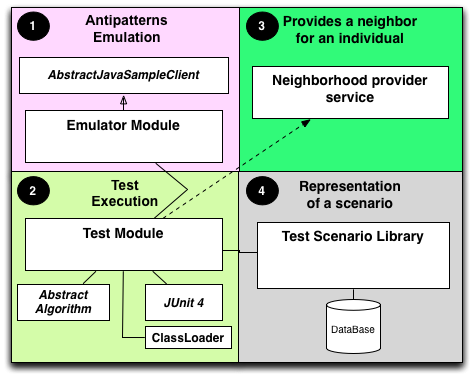
\includegraphics[width=0.5\textwidth]{./images/testbedarch.png}
\caption{Testbed main architecture.}
\label{fig:testbedarch}
\end{figure} 

\begin{figure}[h]
\centering
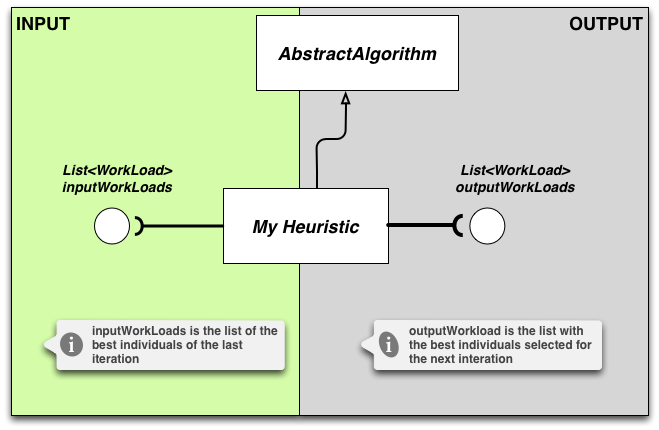
\includegraphics[width=0.5\textwidth]{./images/myheuristic.png}
\caption{Test Module class diagram.}
\label{fig:heuristicclassdiagram}
\end{figure} 



\subsection{Test Module}

The Test Module is responsible for load all classes that extends AbstractAlgorithm in the classpath and perform the tests under the application. The Emulator Module provides successful scenarios and antipatterns implementations. The heuristics are executed in order to select the scenarios with failures or high response times. 

\begin{figure}[h]
\begin{minipage}{.5\textwidth}
\centering
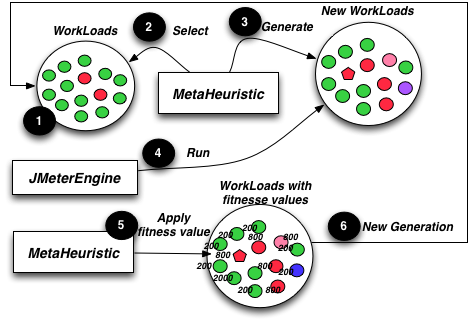
\includegraphics[width=1\textwidth]{./images/step2.png}
\caption{Test Module life cycle.}
\label{fig:step2}
\end{minipage}
\end{figure} 

The Fig. \ref{fig:step2} presents the Test Module life cycle. The life cycle iterate over two steps: The first step apply a metaheurist to select or generate a new set of workloads based on selection criteria. The second step run each workload with the JMeterEngine and obtain a fitness value based on some objective function. The red circles represent the workload that contain errors. The green circles represents the workloads with no errors and low acceptable response time.  Each Metaheuristic could define your own objective function. After all these steps the cycle begins until the maximum number of generations it is reached. 

The Fig. \ref{fig:heuristicclassdiagram} shows the  class diagram for custom and provided heuristics. All heuristic classes extends the class AbstractAlgorithm. The heuristics receives  as input a  list of workloads and a list of testcases. Each workload represent an individual in the search space. Each metaheuristic class returns a list of workloads (the individuals selected to the next generation). 



\subsection{Emulator Module}

The Emulator Module is responsible for implement and provide successful scenarios and the most commons performance antipatterns (Figure \ref{fig:testbedarch}  -\ding{202}). All classes must extends the AbstractJavaSamplerClient class or use JUnit 4. The AbstractJavaSamplerClient class allows create a JMeter Java Request.  Using JUnit 4, the emulators classes could be called by a JMeter JUnit request, an Apache JMeter module responsible for unit tests. The Fig. \ref{fig:emulator} presents the main features of the emulator module. The module implements 8 test scenarios in its first version.

\begin{figure}[h]
\centering
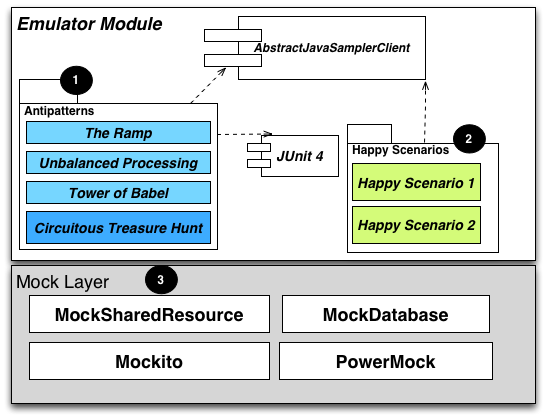
\includegraphics[width=0.4\textwidth]{./images/emulator.png}
\caption{Emulator module}
\label{fig:emulator}
\end{figure}  

The Mock Layer provides emulated databases and components to the test scenarios. Each scenario provided by the Emulator Module could be called in JMeter using a Java Request. 

\subsection{Test Scenario Library}

This modules provides a common representation. The representation for all scenarios. Each scenario is composed by a linear vector with 23 positions. The first position represents the name of an individual. The second position represents the algorithm (genetic algorithm, simulated annealing, or Tabu search) used by the individual. The third position represents the type of test (load, stress, or performance). The next positions represent 10 scenarios and their numbers of users. Each scenario is an atomic operation: the scenario must log into the application, run the task goal, and undo any changes performed, returning the application to its original state.

Fig. \ref{fig:genomarepresentation} presents the solution representation and an example using the crossover operation. In the example, genotype 1 has the Login scenario with 2 users, the Form scenario with 0 users, and the Search scenario with 3 users. Genotype 2 has the Delete scenario with 10 users, the Search scenario with 0 users, and the Include scenario with 5 users. After the crossover operation, we obtain a genotype with the Login scenario with 2 users, the Search scenario with 0 users, and the Include scenario with 5 users.

\begin{figure}[h]
\centering
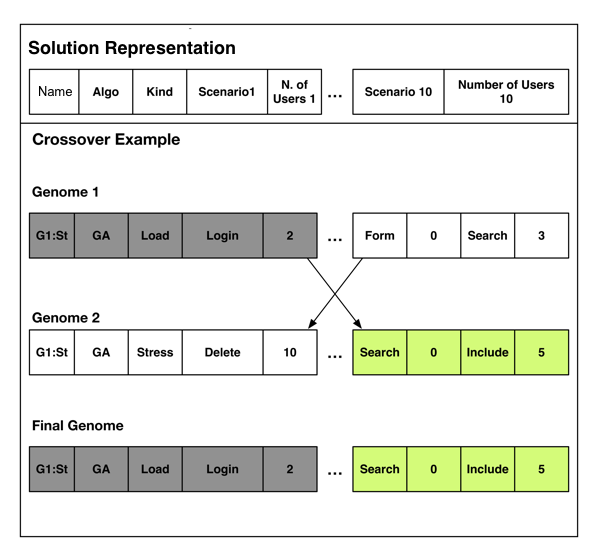
\includegraphics[width=0.5\textwidth]{./images/genomerepresentation1.png}
\caption{Solution representation and crossover example}
\label{fig:genomarepresentation}
\end{figure}


\subsection{Neighborhood provider service}


Fig. \ref{fig:neighbourtaby} shows the strategy used by the proposed solution to obtain the representation of the neighbors for the Tabu search and simulated annealing algorithms. The neighbors are obtained by the modification of a single position (scenario or number of users) in the vector.


\begin{figure}[h]
\centering
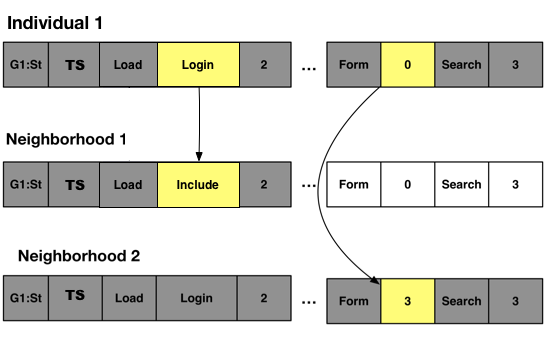
\includegraphics[width=0.4\textwidth]{./images/neighbor.png}
\caption{Neighborhood provider strategy}
\label{fig:neighbourtaby}
\end{figure}



\section{Experiments}

In this section, We present the results of experiments which we carried out to verify the antipatterns  implementation and the metaheuristics used by the testbed tool. We conducted two experiments in order to verify the effectiveness of the testbed tool.

The scope of the experiments is analyze the use of the IAdapter testbed  for the purpose of evaluation with respect to effectiveness and efficienct from the point of view of the tester in the context of  stress test  practices.  The experiments ran for 17 generations. The experiments used an initial population of 4 individuals by metaheuristic. The genetic algorithm used the top 10 individuals from each generation in the crossover operation. The Tabu list was configured with the size of 10 individuals and expired every 2 generations.  The mutation operation was applied to 10\% of the population on each generation. The experiments uses tabu search, genetic algorithms and the hybrid metaheuristic approach proposed by Gois et al. \cite{Gois2016}. The objective function applied is intended to maximize the number of users and minimize the response time of the scenarios being tested.  In this experiments, better fitness values meaning to find scenarios with more users and a low values of response time. A penalty is applied when the response time is greater than the  maximum response time expected. 

\subsection{Research Questions}

The following research question is addressed:
\begin{itemize}
\item Does the IAdapter testbed reproduce a workload by using an antipattern implementation?
\item Does the IAdapter testbed be able to provide client and server metrics with the aim of being used for web performance evaluation studies?
\item The IAdapter testbed should be extensible, allowing create new test scenarios?
\end{itemize}

\subsection{Variables}

The independent variables are the test scenarios (antipatterns and happy scenarios). The dependent variable are the maximal number of users supported by the application.

\subsection{The Ramp and Circuitous Treasure Hunt experiment}

The experiment was carried out for 8 continuous hours.  All tests in the experiment were conducted without the need of a tester, automating the process of executing and designing performance test scenarios.In this experiment, Scenarios were generated with the Ramp and Circuitous Treasure antipattern as well as scenarios with Happy Scenario 1, Happy Scenario 2 and mixed scenarios. The Fig. \ref{fig:fitnessbygeneration1} and \ref{fig:fitnessbygeneration1-2} presents the fitness value obtained by each metaheuristic. The SA algorithm obtained the worst fitness values. Hybrid metaheuristic obtained the better fitness values. 


\begin{figure}[h]
\begin{minipage}{.5\textwidth}
\centering
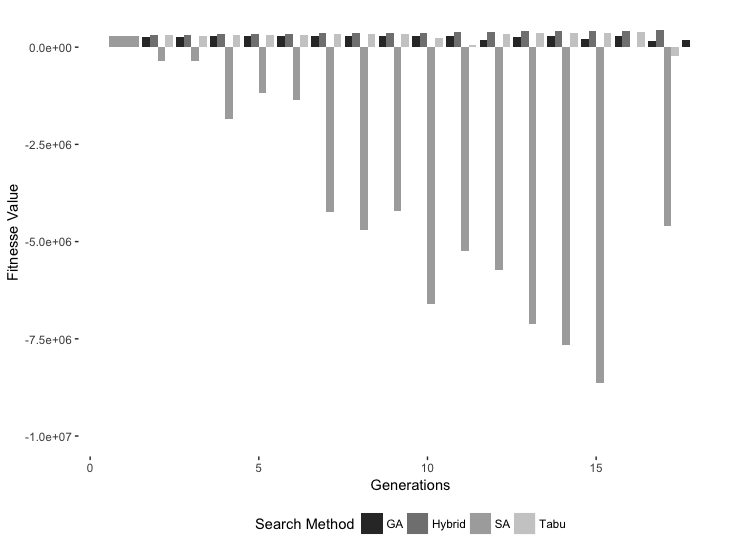
\includegraphics[width=1\textwidth]{./images/experiment1-1-bw.png}
\caption{fitness value obtained by Search Method }
\label{fig:fitnessbygeneration1}
\end{minipage}
\begin{minipage}{.5\textwidth}
\centering
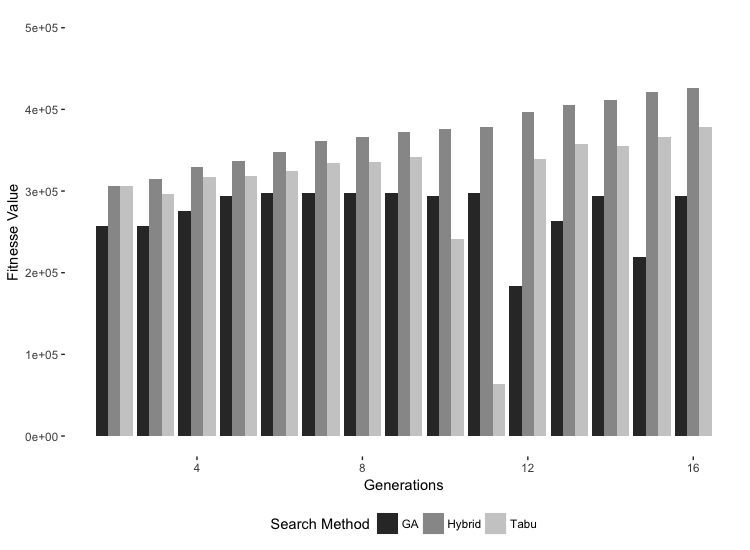
\includegraphics[width=1\textwidth]{./images/experiment1-2-bw.png}
\caption{fitness value obtained by Search Method without SA metaheuristic.}
\label{fig:fitnessbygeneration1-2}
\end{minipage}
\end{figure}

Despite having obtained the best fitness value in each generation, the Hybrid algorithm performs twice as many requests as the second one, the tabu search (Fig. \ref{fig:numberofrequestsbysearchmethod}). The Fig. \ref{fig:boxplot1} shows the average, minimal e maximum value by search method.


\begin{figure}[h]
\begin{minipage}{.5\textwidth}
\centering
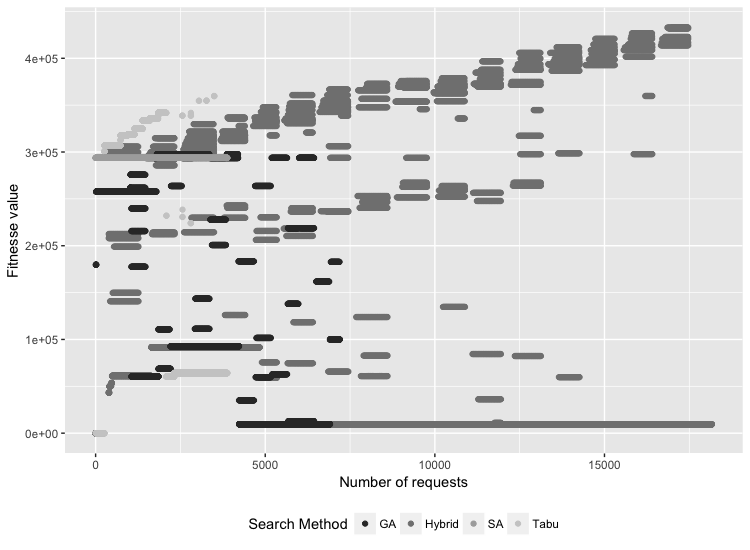
\includegraphics[width=1\textwidth]{./images/experiment1-3-bw.png}
\caption{Number of requests by Search Method}
\label{fig:numberofrequestsbysearchmethod}
\end{minipage}
\begin{minipage}{.5\textwidth}
\centering
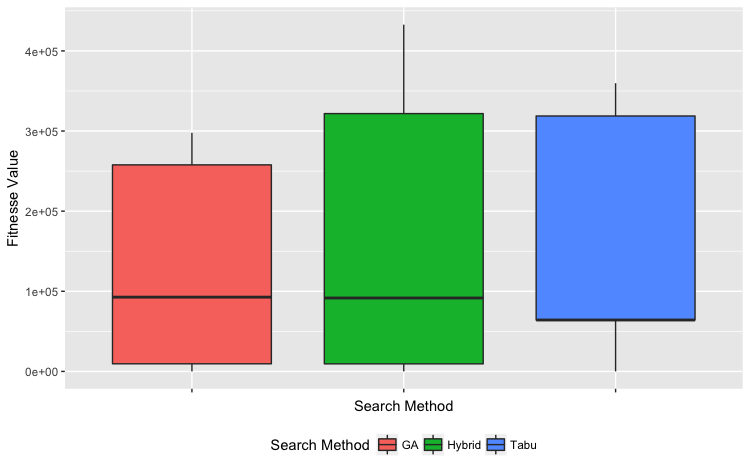
\includegraphics[width=1\textwidth]{./images/experiment1-4.png}
\caption{Average, median, maximum and minimal fitness value by Search Method}
\label{fig:boxplot1}
\end{minipage}
\end{figure}

The Fig. \ref{fig:summaryboxplot1} presents the maximum, average, median and minimum fitness value by generation. The maximun fitness value increases at each generation. The Fig. \ref{fig:density1} presents the density graph of number of users by fitness value. The range between 100 and 150 users has the highest number of individuals found with higher fitness value.

\begin{figure}[h]
\begin{minipage}{.5\textwidth}
\centering
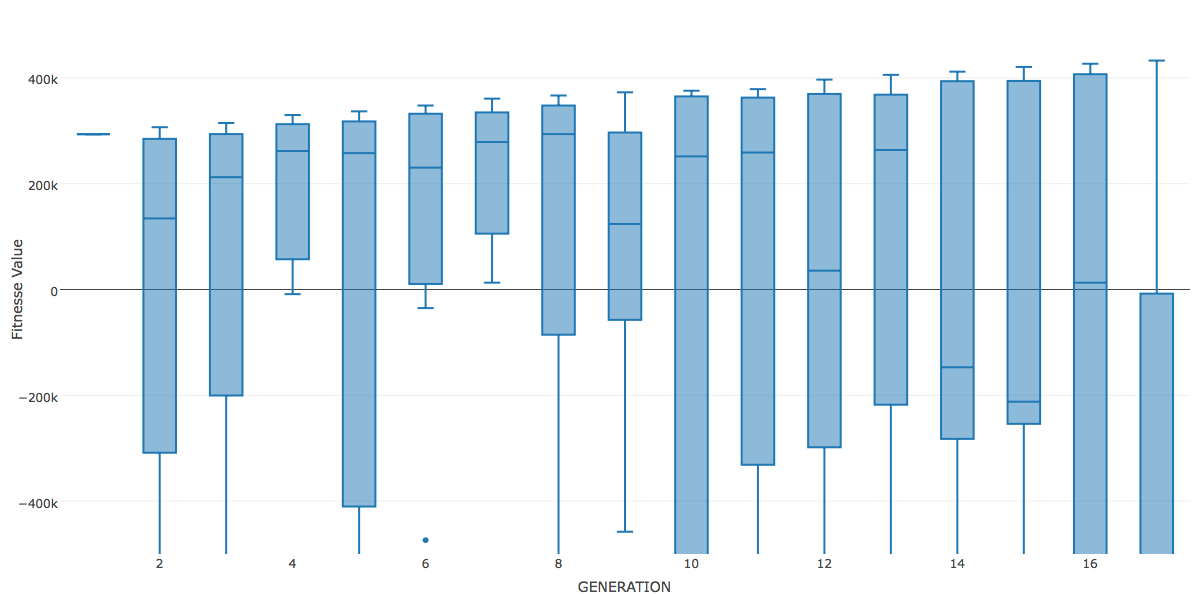
\includegraphics[width=1\textwidth]{./images/experiment1-5.png}
\caption{fitness value by generation}
\label{fig:summaryboxplot1}
\end{minipage}
\begin{minipage}{.5\textwidth}
\centering
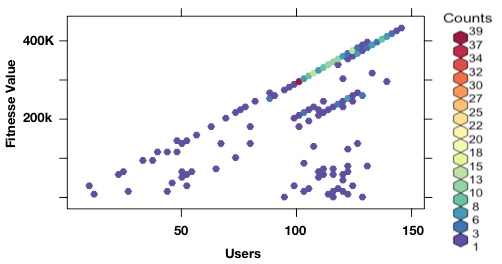
\includegraphics[width=1\textwidth]{./images/experiment1-6.png}
\caption{Density graph of number of users by fitness value}
\label{fig:density1}
\end{minipage}
\end{figure}

Table \ref{tab:bestindividuals} shows 4 individuals with 143 to 146 users. These are the scenarios with the maximum number of users found with the best response time. The first individual has 64 users on Happy Scenario 2, 81 users on Happy Scenario 1 and a response time of 12 seconds. None of the best individuals has one of the antipatterns used in the experiment.



% Please add the following required packages to your document preamble:
% \usepackage[table,xcdraw]{xcolor}
% If you use beamer only pass "xcolor=table" option, i.e. \documentclass[xcolor=table]{beamer}
\begin{table}[h]
\centering
\caption{Best individuals found in the first experiment}
\label{tab:bestindividuals}
\begin{tabular}{lllllll}
\rowcolor[HTML]{C0C0C0} 
\textbf{Search Method} & \textbf{Generation} & \textbf{Users} & \textbf{fitness Value} & \textbf{Happy 2} & \textbf{Happy 1} & \textbf{Response Time} \\
Hybrid & 17 & 145 & 432760 & 64 & 81 & 12 \\
Hybrid & 17 & 145 & 432740 & 46 & 99 & 13 \\
Hybrid & 17 & 146 & 431760 & 54 & 92 & 12 \\
Hybrid & 16 & 143 & 426740 & 30 & 113 & 13
\end{tabular}
\end{table}

Fig. \ref{fig:responsetimegenerationalltests1} presents the response time by number of users of individuals with Happy Scenario 1 and Happy Scenario 2. The Figure illustrates that the individuals with best fitness value has more users and minor response time. The Fig. \ref{fig:fitnessgenerationalltests1-1} presents the response time by number of users of individuals with the Ramp and Circuitous Treasure antipatterns scenarios. The Figure illustrates the smallest number of individuals with the antipatterns when compared to individuals who use the happy scenarios.


\begin{figure}[h]
\begin{minipage}{.5\textwidth}
\centering
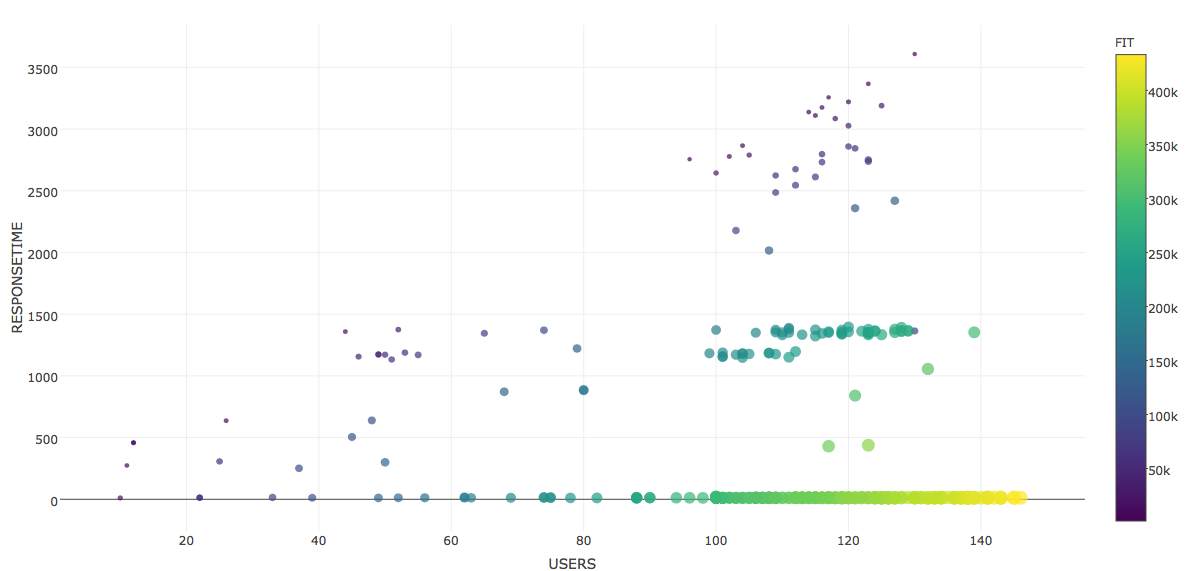
\includegraphics[width=1\textwidth]{./images/experiment1-7.png}
\caption{Response time by number of users of individuals with Happy Scenario 1 and Happy Scenario 2}
\label{fig:responsetimegenerationalltests1}
\end{minipage}
\begin{minipage}{.5\textwidth}
\centering
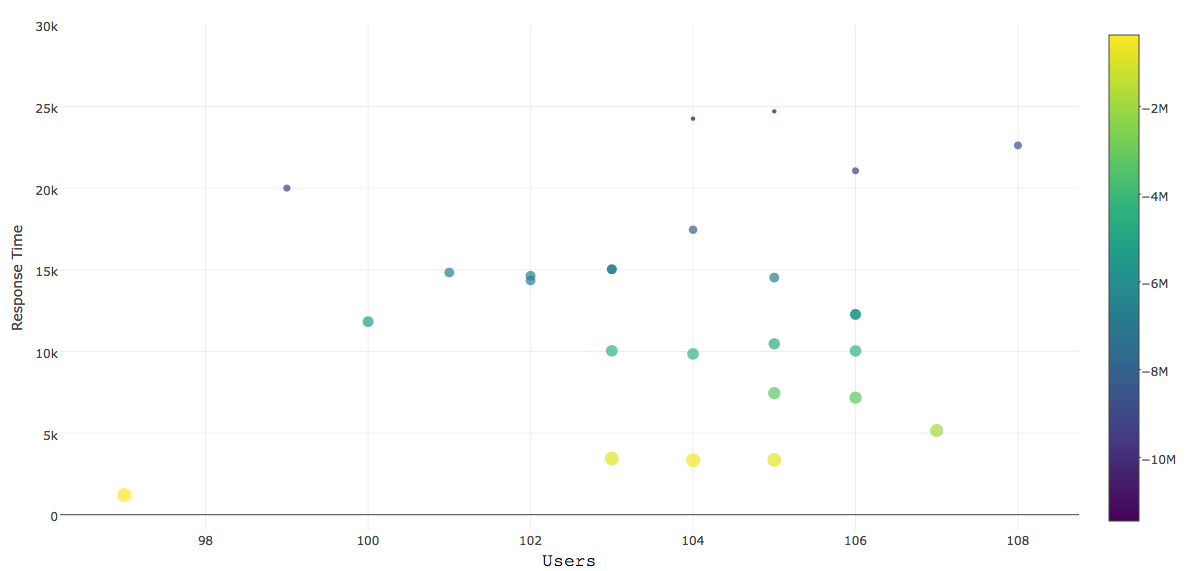
\includegraphics[width=1\textwidth]{./images/experiment1-8.png}
\caption{Response time by number of users of individuals with the Ramp and Circuitous Treasure antipatterns}
\label{fig:fitnessgenerationalltests1-1}
\end{minipage}
\end{figure}

In the first experiment, We conclude that the metaheuristics converged to scenarios with an happy path, excluding the scenarios with antipatterns. The hybrid metaheuristic returned individuals with higher fitness scores. However, the Hybrid metaheuristic made twice as many requests than Tabu Search to overcome it. The SA algorithm obtained the worst fitness values. The algorithm initially used a scenario with the Ramp and Circuitous Treasure antipatterns  and found neighbors that still using the antipatterns over the 17 generations of the experiment.





\subsection{The Tower Babel  and Unbalanced Processing experiment}

The experiment was carried out for 6 continuous hours. All tests in the experiment were conducted without the need of a tester. In this experiment, Scenarios were generated with Tower Babel and Unbalanced Processing antipattern as well as scenarios with Happy Scenario 1, Happy Scenario 2 and mixed scenarios. The Fig. \ref{fig:fitnessbygeneration2}  presents the fitness value obtained by each metaheuristic. The SA algorithm obtained the worst fitness values. Hybrid metaheuristic obtained the better fitness values.


\begin{figure}[h]
\centering
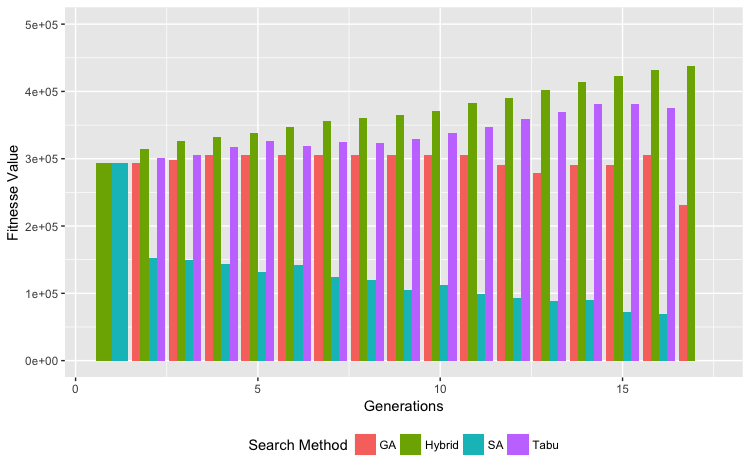
\includegraphics[width=.7\textwidth]{./images/experiment2-7.png}
\caption{itnesse value obtained by Search Method}
\label{fig:fitnessbygeneration2}
\end{figure}

As in the first experiment, the Hybrid algorithm performs twice as many requests as the second one, the tabu search (Fig. \ref{fig:numberofrequestsbysearchmethod2}). The Fig. \ref{fig:boxplot2} shows the average, minimal e maximum value by search method. The Fig. \ref{fig:summaryboxplot2} presents the maximum, average, median and minimum fitness value by generation. The maximun fitness value increases at each generation. The Fig. \ref{fig:density2} presents the density graph of number of users by fitness value. The range between 100 and 150 users has the highest number of individuals found with higher fitness value.


\begin{figure}[h]
\begin{minipage}{.5\textwidth}
\centering
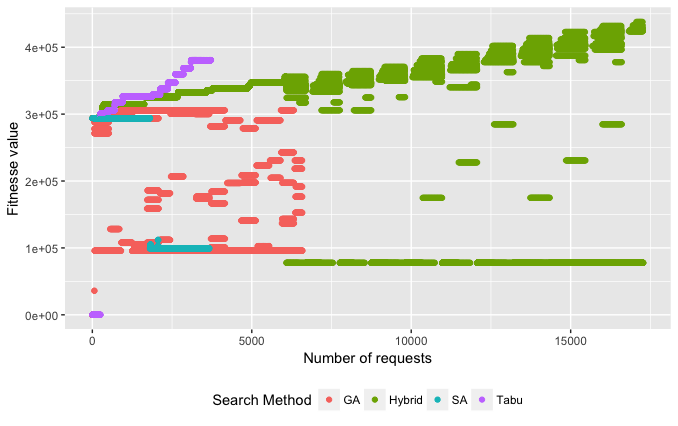
\includegraphics[width=1\textwidth]{./images/experiment2-1.png}
\caption{Number of requests by Search Method}
\label{fig:numberofrequestsbysearchmethod2}
\end{minipage}
\begin{minipage}{.5\textwidth}
\centering
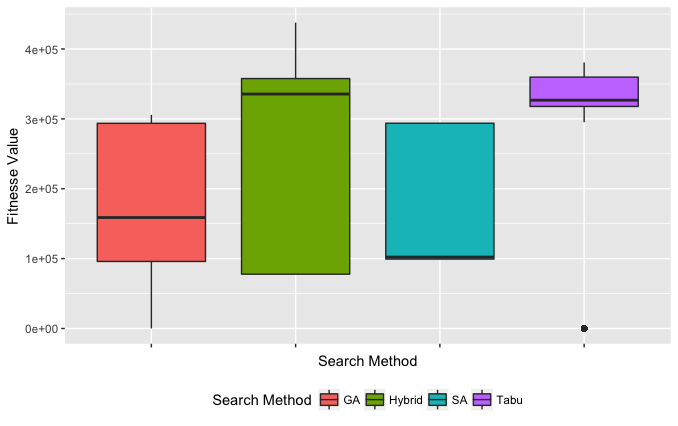
\includegraphics[width=1\textwidth]{./images/experiment2-2.png}
\caption{Finesse value by generation in all tests}
\label{fig:boxplot2}
\end{minipage}

\end{figure}



\begin{figure}[h]
\begin{minipage}{.5\textwidth}
\centering
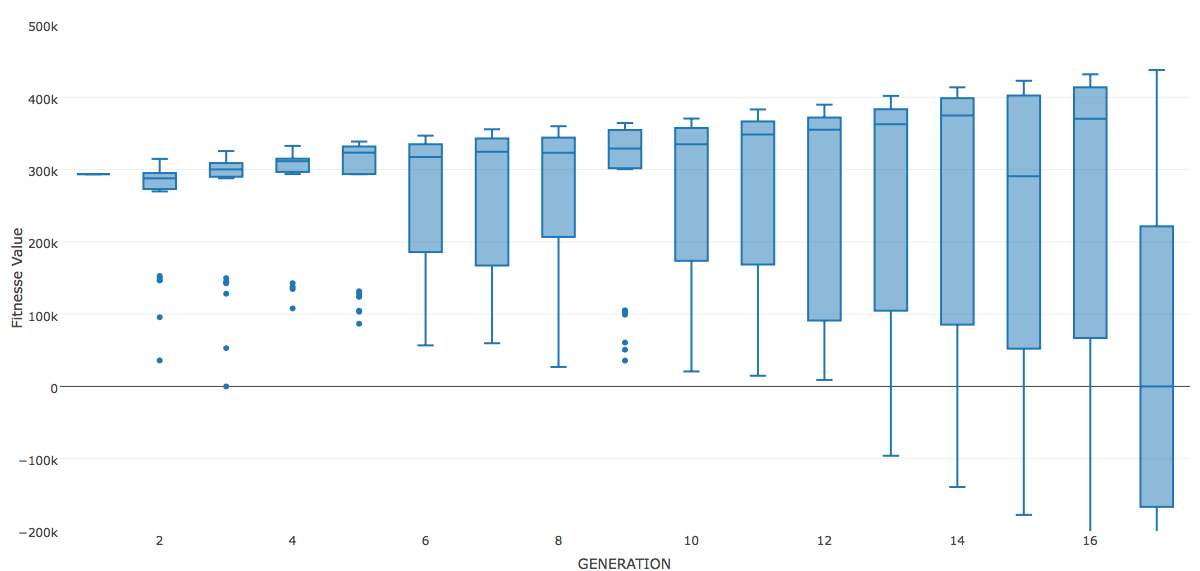
\includegraphics[width=1\textwidth]{./images/experiment2-3.png}
\caption{Response time by generation in all tests scenarios}
\label{fig:summaryboxplot2}
\end{minipage}
\begin{minipage}{.5\textwidth}
\centering
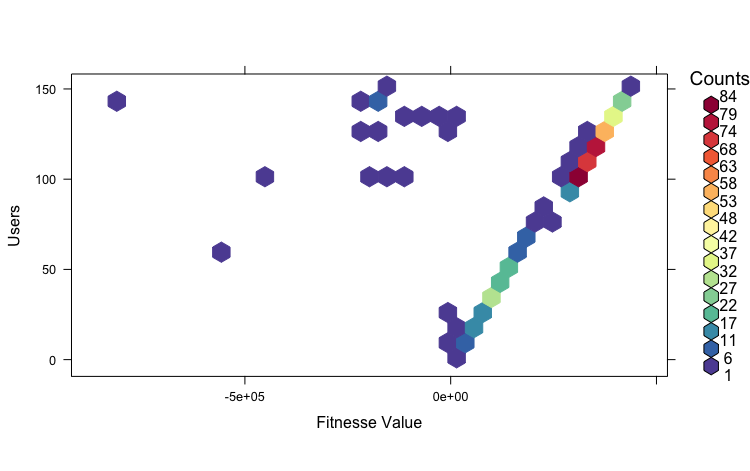
\includegraphics[width=1\textwidth]{./images/experiment2-4.png}
\caption{Density graph of number of users by fitness value}
\label{fig:density2}
\end{minipage}

\end{figure}

Table \ref{tab:bestindividuals2} shows 4 individuals with 145 to 148 users.  The first individual has 72 users on Happy Scenario 2, 30 users on Happy Scenario 1, 46 user with the antipattern Tower Babel and a response time of 11 seconds. Despite the fact of doing 300 conversions of the JSON standard for XML. The antipattern implementation does not return a much higher response time than happy paths. While happy paths returns from 10 to 15 seconds from a single user, Tower Babel antipattern has a response time of 10 to 29 seconds. None of the best individuals found implements the Unbalanced Processing antipattern.

Fig. \ref{fig:responsetimegenerationalltests2} presents the response time by number of users of individuals with Happy Scenario 1 and Happy Scenario 2. The Figure illustrates that the individuals with best fitness value has more users and minor response time. The Fig. \ref{fig:fitnessgenerationalltests2-1} presents the response time by number of users of individuals with with Unbalanced Processing antipatterns scenarios. The Figure illustrates the smallest number of individuals with the  Unbalanced Processing antipattern when compared to individuals who use the happy scenarios and the Tower Babel antipattern.



\begin{figure}[h]
\centering
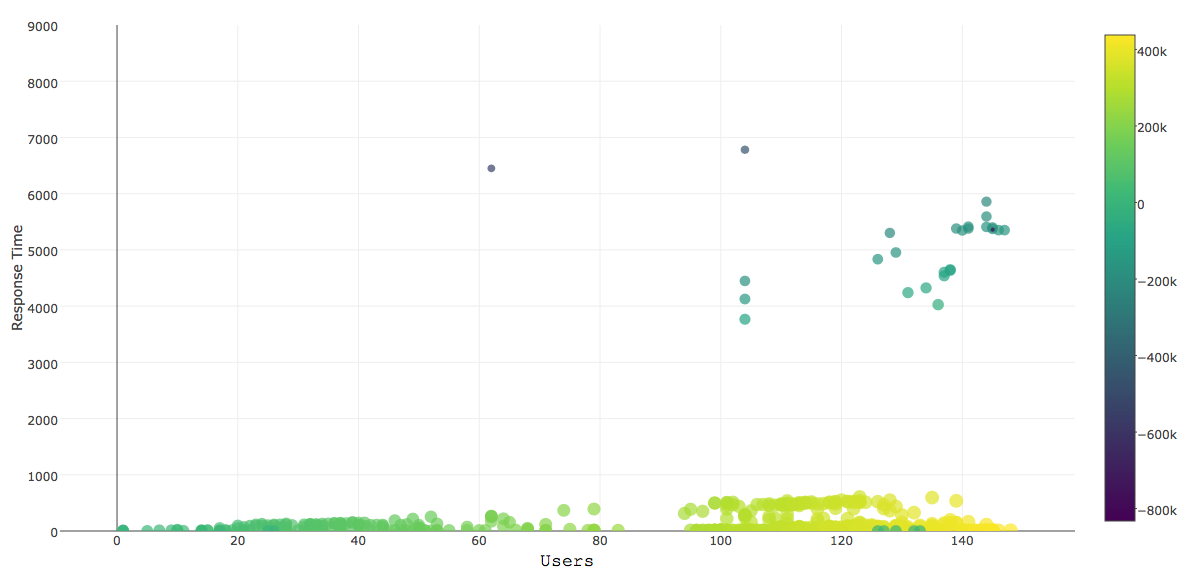
\includegraphics[width=0.7\textwidth]{./images/experiment2-5.png}
\caption{Response time by number of users of individuals with Happy Scenario 1, Happy Scenario 2 and Tower Babel antipattern}
\label{fig:responsetimegenerationalltests2}
\end{figure}


\begin{figure}[h]
\centering
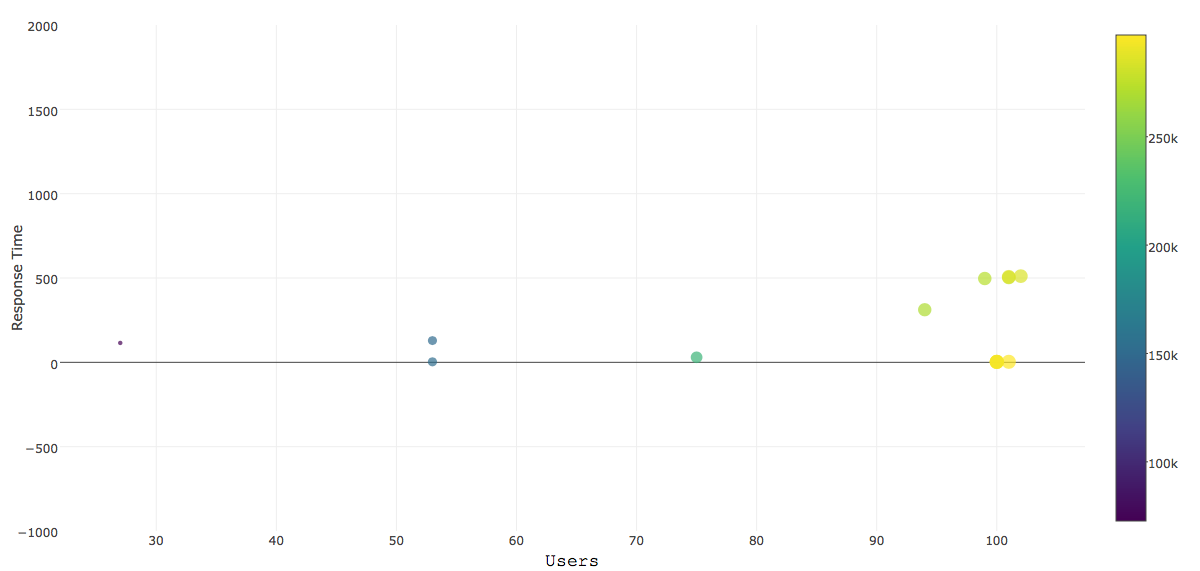
\includegraphics[width=0.7\textwidth]{./images/experiment2-6.png}
\caption{Response time by number of users of individuals with Unbalanced Processing antipattern}
\label{fig:fitnessgenerationalltests2-1}
\end{figure}


We conclude that the metaheuristics converged to scenarios with an happy path and Tower Babel antipattern, excluding the scenarios with Unbalanced Processing antipattern. The hybrid metaheuristic returned individuals with higher fitness scores. However, the Hybrid metaheuristic made twice as many requests than Tabu Search to overcome it. The SA algorithm obtained the worst fitness values. The algorithm initially used a scenario with an antipattern and found neighbors that still using an antipattern over the 17 generations of the experiment. The individual with best fitness value has 72 users on Happy Scenario 2, 30 users on Happy Scenario 1, 46 user with the antipattern Tower Babel and a response time of 11 seconds.

% Please add the following required packages to your document preamble:
% \usepackage[table,xcdraw]{xcolor}
% If you use beamer only pass "xcolor=table" option, i.e. \documentclass[xcolor=table]{beamer}
\begin{table}[h]
\centering
\caption{Best individuals found in the second experiment}
\label{tab:bestindividuals2}
\begin{tabular}{llllllll}
\rowcolor[HTML]{FFCCC9} 
\textbf{Search Method} & \textbf{Generation} & \textbf{Users} & \textbf{fitness Value} & \textbf{Happy 2} & \textbf{Tower} & \textbf{Happy 1} & \textbf{Time} \\ 
\multicolumn{1}{l}{Hybrid} & \multicolumn{1}{l}{17} & \multicolumn{1}{l}{148} & \multicolumn{1}{l}{437780} & \multicolumn{1}{l}{72} & \multicolumn{1}{l}{46} & \multicolumn{1}{l}{30} & \multicolumn{1}{l}{11} \\ 
\multicolumn{1}{l}{Hybrid} & \multicolumn{1}{l}{17} & \multicolumn{1}{l}{145} & \multicolumn{1}{l}{432740} & \multicolumn{1}{l}{71} & \multicolumn{1}{l}{15} & \multicolumn{1}{l}{59} & \multicolumn{1}{l}{13} \\ 
\multicolumn{1}{l}{Hybrid} & \multicolumn{1}{l}{16} & \multicolumn{1}{l}{146} & \multicolumn{1}{l}{431800} & \multicolumn{1}{l}{72} & \multicolumn{1}{l}{31} & \multicolumn{1}{l}{43} & \multicolumn{1}{l}{10} \\ 
\multicolumn{1}{l}{Hybrid} & \multicolumn{1}{l}{17} & \multicolumn{1}{l}{145} & \multicolumn{1}{l}{428780} & \multicolumn{1}{l}{71} & \multicolumn{1}{l}{32} & \multicolumn{1}{l}{42} & \multicolumn{1}{l}{11} \\ 
\end{tabular}
\end{table}

\section{Conclusion}

IAdapter Testbed is an open-source facility that provides software tools for search based test research. The testbed tool emulates test scenarios in a controled environment using mock objects and implementing performance antipatterns.  Two experiments were conducted to validate the proposed approach. The experiments uses genetic, algorithms, tabu search, simulated annealing and an hybrid approach proposed by Gois et al. \cite{Gois2016}.

The experiments ran for 17 generations. The experiments used an initial population of 4 individuals by metaheuristic. All tests in the experiment were conducted without the need of a tester, automating the execution of stress tests with the JMeter tool.

In both experiments the hybrid metaheuristic returned individuals with higher fitness scores. However, the Hybrid metaheuristic made twice as many requests than Tabu Search to overcome it. The SA algorithm obtained the worst fitness values. The algorithm initially used a scenario with an antipattern and found neighbors that still using the antipatterns over the 17 generations of the experiment.

In the first experiment the metaheuristics converged to scenarios with an happy path, excluding the scenarios with the use of an antipatterns. The individual with best fitness value has 64 users on Happy Scenario 2, 81 users on Happy Scenario 1 and a response time of 12 seconds. None of the best individuals has one of the antipatterns used in the experiment.


In the second experiment,  the metaheuristics converged to scenarios with an happy path and Tower Babel antipattern, excluding the scenarios with Unbalanced Processing antipattern. The individual with best fitness value has 72 users on Happy Scenario 2, 30 users on Happy Scenario 1, 46 user with the antipattern Tower Babel and a response time of 11 seconds. Future works include the use of new antipatterns and more experiments with the use of the antipattern Tower Babel.

